\subsection{Interrelación Asesor - Alumno Curso Académico}

   \begin{description}
      \item[Definición] En esta interrelación se deja constancia de que un
      asesor puede ofrecer servicios de asesoría a un número indeterminado
      de alumnos matriculados durante un determinado curso académico.

      \item[Características] La interrelación presenta las siguientes
                             características:

         \begin{itemize}
            \item \textbf{Nombre:} As-AlCA
            \item \textbf{Tipo de la interrelación:} El tipo de entidad
                  Alumno Curso Académico es débil por existencia respecto al
                  tipo de entidad Asesor.
            \item \textbf{Cardinalidad de la interrelación:} 1:N
            \item \textbf{Número de atributos:} Ninguno.
         \end{itemize}

      \item[Diagrama] La figura \ref{diagramaAs-AlCA} muestra el diagrama de la
                      interrelación.

      \item \begin{figure}[!ht]
            \begin{center}
            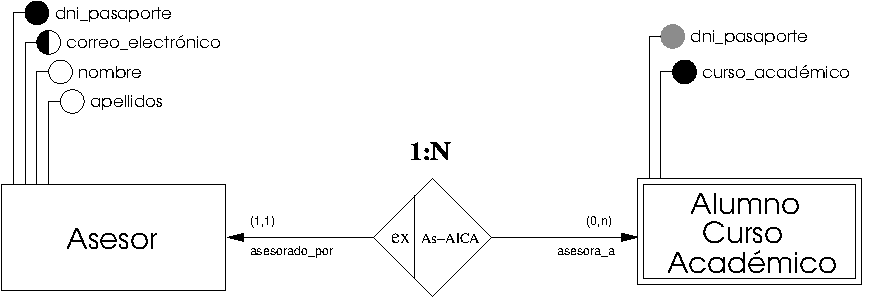
\includegraphics[]{07.Modelo_Entidad-Interrelacion/7.3.Analisis_Interrelaciones/diagramas/As-AlCA.pdf}
            \caption{Diagrama de la interrelación As-AlCA.}
            \label{diagramaAs-AlCA}
            \end{center}
         \end{figure}

      \item[Ejemplo práctico del tipo de interrelación]

      \item \begin{center}
            \begin{tabular}{ | r r | }
            \hline
            \multicolumn{2}{ | c | }{\textbf{Tipo de interrelación As-AlCA}} \\
            \hline
            \textbf{Asesor} & \\
            dni\_pasaporte & 98765432Z \\
            \hline
            \textbf{Alumno Curso Académico} & \\
            dni\_pasaporte & 01234567A \\
            id\_centro & 2008 \\
            \hline
            \end{tabular}
         \end{center}
   \end{description}
